% Espacios horizontal y vertical en fibrados
% Compilar con: pdflatex horizontal_vertical.tex
\documentclass[tikz,border=10pt]{standalone}
\usepackage{tikz}
\usepackage{amsmath}
\usepackage{xcolor}
\definecolor{gdlblue}{RGB}{41, 98, 168}
\definecolor{gdlred}{RGB}{191, 49, 49}
\definecolor{gdlgreen}{RGB}{30, 130, 76}
\definecolor{gdlorange}{RGB}{217, 130, 30}
\definecolor{gdlpurple}{RGB}{118, 56, 138}
\definecolor{gdlgray}{RGB}{140, 140, 140}
\definecolor{gdlyellow}{RGB}{190, 140, 10}
\usetikzlibrary{arrows.meta, decorations.pathmorphing, calc, 3d}

\begin{document}
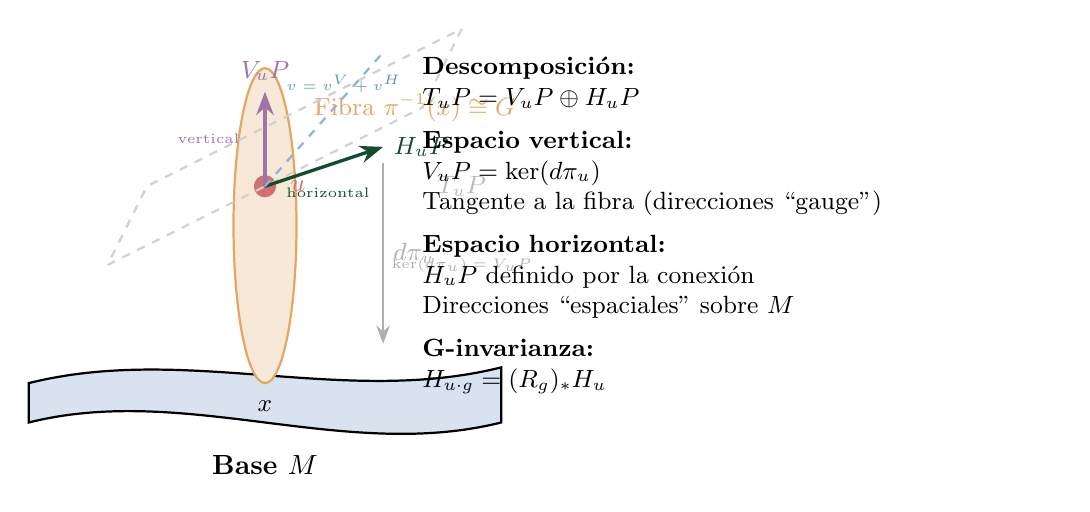
\begin{tikzpicture}[>=Stealth]

% === Fibrado principal ===
% Base M
\begin{scope}[shift={(0, -2)}]
    \draw[thick, fill=gdlblue!18]
        (-3, 0) .. controls (-1, 0.5) and (1, -0.3) .. (3, 0.2) --
        (3, -0.5) .. controls (1, -1) and (-1, 0) .. (-3, -0.5) -- cycle;
    \node[below] at (0, -0.8) {\textbf{Base $M$}};

    % Punto x
    \fill[gdlblue!70] (0, 0.1) circle (3pt);
    \node[below, font=\small] at (0, -0.1) {$x$};
\end{scope}

% Fibra sobre x
\draw[thick, gdlorange!70, fill=gdlorange!18] (0, 0) ellipse (0.4cm and 2cm);
\node[gdlorange!70, right, font=\small] at (0.5, 1.5) {Fibra $\pi^{-1}(x) \cong G$};

% Punto u en la fibra
\fill[gdlred!70] (0, 0.5) circle (4pt);
\node[right, font=\small, gdlred!70] at (0.2, 0.5) {$u$};

% === Espacio tangente en u ===
\begin{scope}[shift={(0, 0.5)}]
    % Plano tangente (sugerido)
    \draw[thick, dashed, gdlgray!40] (-2, -1) -- (2, 1) -- (2.5, 2) -- (-1.5, 0) -- cycle;
    \node[gdlgray!60, font=\small] at (2.5, 0) {$T_u P$};

    % Espacio vertical (tangente a la fibra)
    \draw[->, very thick, gdlpurple!70] (0, 0) -- (0, 1.2) node[above, font=\small] {$V_u P$};
    \node[gdlpurple!70, font=\tiny, left] at (-0.2, 0.6) {vertical};

    % Espacio horizontal (complemento)
    \draw[->, very thick, gdlgreen!60!black] (0, 0) -- (1.5, 0.5) node[right, font=\small] {$H_u P$};
    \node[gdlgreen!60!black, font=\tiny, below] at (0.8, 0.1) {horizontal};

    % Descomposición
    \draw[thick, dashed, gdlblue!50] (0, 0) -- (1.5, 1.7);
    \node[gdlblue!70, font=\tiny] at (1, 1.3) {$v = v^V + v^H$};
\end{scope}

% === Proyección d\pi ===
\draw[->, thick, gdlgray!70] (1.5, 0.8) -- node[right, font=\small] {$d\pi_u$} (1.5, -1.5);
\node[gdlgray!70, font=\tiny] at (2.5, -0.5) {$\ker(d\pi_u) = V_u P$};

% === Propiedades ===
\node[font=\small, text width=8cm] at (6, 0) {
    \textbf{Descomposición:}\\
    $T_u P = V_u P \oplus H_u P$\\[0.5em]
    \textbf{Espacio vertical:}\\
    $V_u P = \ker(d\pi_u)$\\
    Tangente a la fibra (direcciones ``gauge'')\\[0.5em]
    \textbf{Espacio horizontal:}\\
    $H_u P$ definido por la conexión\\
    Direcciones ``espaciales'' sobre $M$\\[0.5em]
    \textbf{G-invarianza:}\\
    $H_{u \cdot g} = (R_g)_* H_u$
};

\end{tikzpicture}
\end{document}
